\documentclass{standalone}
\usepackage{tikz}
\usetikzlibrary{patterns, positioning}

\begin{document}
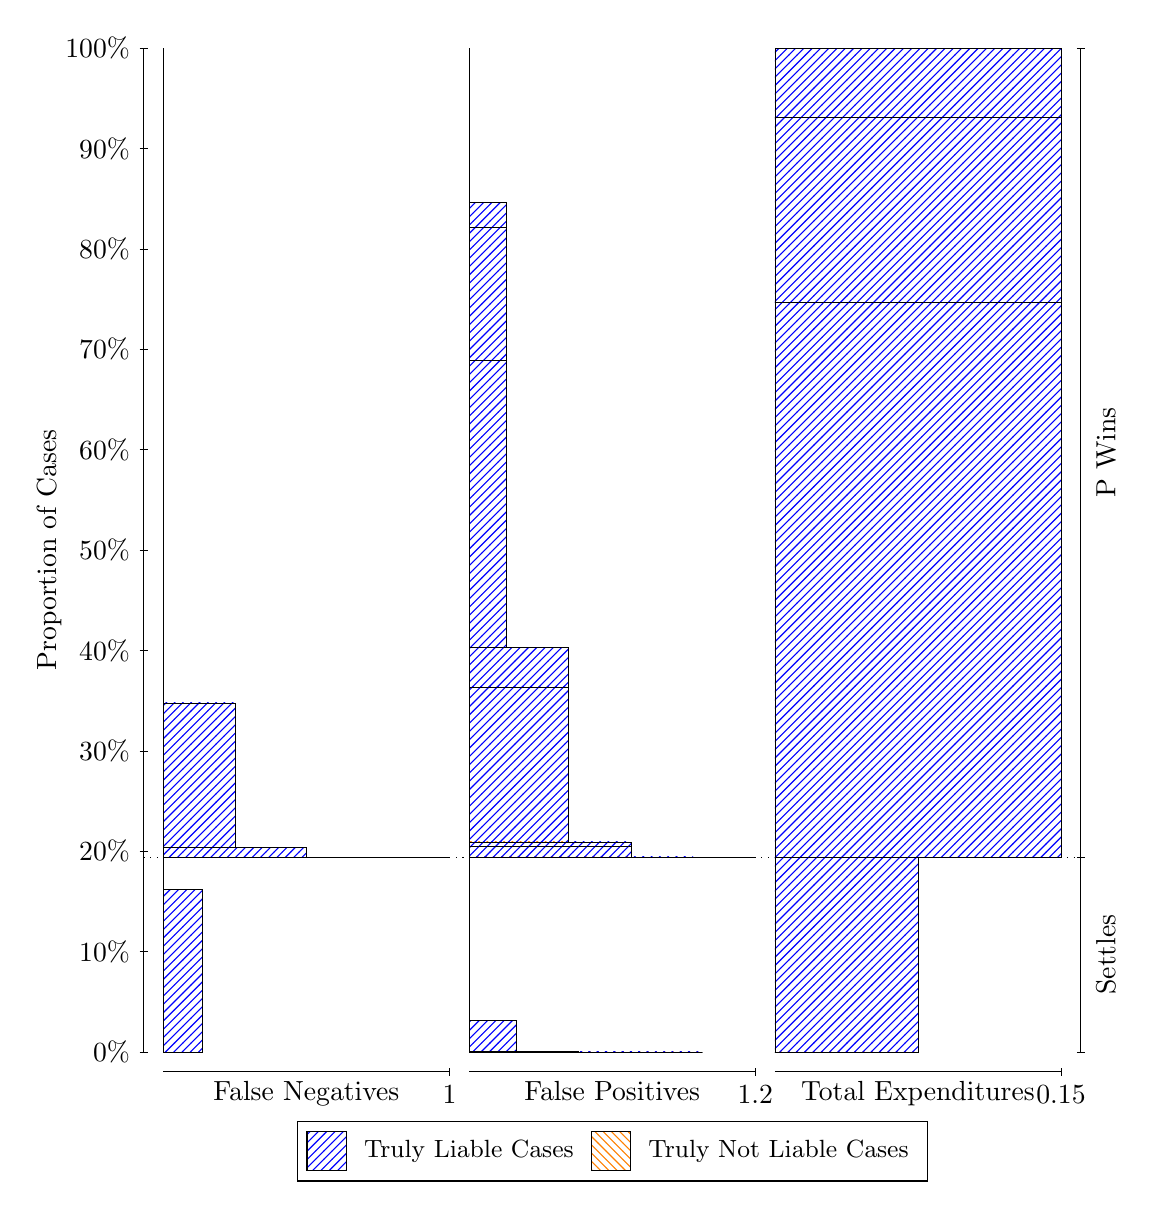
\begin{tikzpicture}
\draw[black, very thin] (1.5,1.75) -- (1.5,14.5);
\node[rotate=90, anchor=center] at (0.3, 8.125) {Proportion of Cases};
\draw[black, very thin] (1.45,1.75) -- (1.55,1.75);
\node[anchor=east] at (1.45, 1.75) {0\%};
\draw[black, very thin] (1.45,3.025) -- (1.55,3.025);
\node[anchor=east] at (1.45, 3.025) {10\%};
\draw[black, very thin] (1.45,4.3) -- (1.55,4.3);
\node[anchor=east] at (1.45, 4.3) {20\%};
\draw[black, very thin] (1.45,5.575) -- (1.55,5.575);
\node[anchor=east] at (1.45, 5.575) {30\%};
\draw[black, very thin] (1.45,6.85) -- (1.55,6.85);
\node[anchor=east] at (1.45, 6.85) {40\%};
\draw[black, very thin] (1.45,8.125) -- (1.55,8.125);
\node[anchor=east] at (1.45, 8.125) {50\%};
\draw[black, very thin] (1.45,9.4) -- (1.55,9.4);
\node[anchor=east] at (1.45, 9.4) {60\%};
\draw[black, very thin] (1.45,10.675) -- (1.55,10.675);
\node[anchor=east] at (1.45, 10.675) {70\%};
\draw[black, very thin] (1.45,11.95) -- (1.55,11.95);
\node[anchor=east] at (1.45, 11.95) {80\%};
\draw[black, very thin] (1.45,13.225) -- (1.55,13.225);
\node[anchor=east] at (1.45, 13.225) {90\%};
\draw[black, very thin] (1.45,14.5) -- (1.55,14.5);
\node[anchor=east] at (1.45, 14.5) {100\%};

\draw[black, very thin] (13.4,1.75) -- (13.4,14.5);
\draw[black, very thin] (13.35,1.75) -- (13.45,1.75);
\node[anchor=west] at (13.35, 1.75) {};
\draw[black, very thin] (13.35,4.2242) -- (13.45,4.2242);
\node[anchor=west] at (13.35, 4.2242) {};
\draw[black, very thin] (13.35,14.5) -- (13.45,14.5);
\node[anchor=west] at (13.35, 14.5) {};

\draw[black, very thin, pattern color=blue, pattern=north east lines] (1.75,1.75) rectangle (2.2496,3.8191);
\draw[black, very thin, pattern color=orange, pattern=north west lines] (1.75,3.8191) rectangle (1.75,3.8191);
\draw[black, very thin, pattern color=blue, pattern=north east lines] (1.75,3.8191) rectangle (1.75,4.2242);
\draw[black, very thin, pattern color=blue, pattern=north east lines] (1.75,4.2242) rectangle (5.3833,4.2242);
\draw[black, very thin, pattern color=blue, pattern=north east lines] (1.75,4.2242) rectangle (4.475,4.2254);
\draw[black, very thin, pattern color=blue, pattern=north east lines] (1.75,4.2254) rectangle (3.5667,4.3458);
\draw[black, very thin, pattern color=blue, pattern=north east lines] (1.75,4.3458) rectangle (2.6583,6.1836);
\draw[black, very thin, pattern color=orange, pattern=north west lines] (1.75,6.1836) rectangle (1.75,6.1836);
\draw[black, very thin, pattern color=blue, pattern=north east lines] (1.75,6.1836) rectangle (1.75,14.5);
\draw[black, very thin, pattern color=orange, pattern=north west lines] (5.6333,1.75) rectangle (8.5953,1.75);
\draw[black, very thin, pattern color=blue, pattern=north east lines] (5.6333,1.75) rectangle (8.5953,1.75);
\draw[black, very thin, pattern color=blue, pattern=north east lines] (5.6333,1.75) rectangle (7.8054,1.75);
\draw[black, very thin, pattern color=blue, pattern=north east lines] (5.6333,1.75) rectangle (7.0156,1.7535);
\draw[black, very thin, pattern color=blue, pattern=north east lines] (5.6333,1.7535) rectangle (6.2257,2.1551);
\draw[black, very thin, pattern color=blue, pattern=north east lines] (5.6333,2.1551) rectangle (5.6333,4.2242);
\draw[black, very thin, pattern color=orange, pattern=north west lines] (5.6333,4.2242) rectangle (9.2667,4.2242);
\draw[black, very thin, pattern color=blue, pattern=north east lines] (5.6333,4.2242) rectangle (9.2667,4.2242);
\draw[black, very thin, pattern color=orange, pattern=north west lines] (5.6333,4.2242) rectangle (8.4768,4.2242);
\draw[black, very thin, pattern color=blue, pattern=north east lines] (5.6333,4.2242) rectangle (8.4768,4.2257);
\draw[black, very thin, pattern color=blue, pattern=north east lines] (5.6333,4.2257) rectangle (8.4768,4.2268);
\draw[black, very thin, pattern color=orange, pattern=north west lines] (5.6333,4.2268) rectangle (7.687,4.2268);
\draw[black, very thin, pattern color=blue, pattern=north east lines] (5.6333,4.2268) rectangle (7.687,4.3612);
\draw[black, very thin, pattern color=blue, pattern=north east lines] (5.6333,4.3612) rectangle (7.687,4.4181);
\draw[black, very thin, pattern color=orange, pattern=north west lines] (5.6333,4.4181) rectangle (6.8971,4.4181);
\draw[black, very thin, pattern color=blue, pattern=north east lines] (5.6333,4.4181) rectangle (6.8971,6.3869);
\draw[black, very thin, pattern color=blue, pattern=north east lines] (5.6333,6.3869) rectangle (6.8971,6.8919);
\draw[black, very thin, pattern color=blue, pattern=north east lines] (5.6333,6.8919) rectangle (6.1072,10.533);
\draw[black, very thin, pattern color=orange, pattern=north west lines] (5.6333,10.533) rectangle (6.1072,10.533);
\draw[black, very thin, pattern color=blue, pattern=north east lines] (5.6333,10.533) rectangle (6.1072,12.222);
\draw[black, very thin, pattern color=blue, pattern=north east lines] (5.6333,12.222) rectangle (6.1072,12.541);
\draw[black, very thin, pattern color=blue, pattern=north east lines] (5.6333,12.541) rectangle (5.6333,14.5);
\draw[black, very thin, pattern color=orange, pattern=north west lines] (9.5167,1.75) rectangle (11.333,1.75);
\draw[black, very thin, pattern color=blue, pattern=north east lines] (9.5167,1.75) rectangle (11.333,4.2242);
\draw[black, very thin, pattern color=orange, pattern=north west lines] (9.5167,4.2242) rectangle (13.15,4.2242);
\draw[black, very thin, pattern color=blue, pattern=north east lines] (9.5167,4.2242) rectangle (13.15,11.273);
\draw[black, very thin, pattern color=orange, pattern=north west lines] (9.5167,11.273) rectangle (13.15,11.273);
\draw[black, very thin, pattern color=blue, pattern=north east lines] (9.5167,11.273) rectangle (13.15,13.619);
\draw[black, very thin, pattern color=orange, pattern=north west lines] (9.5167,13.619) rectangle (13.15,13.619);
\draw[black, very thin, pattern color=blue, pattern=north east lines] (9.5167,13.619) rectangle (13.15,14.5);
\draw[black, dotted] (1.5,4.2242) -- (13.4,4.2242);
\draw[black, very thin] (1.75,1.5) -- (5.3833,1.5);
\node[anchor=north] at (3.5667, 1.5) {False Negatives};
\draw[black, very thin] (5.3833,1.45) -- (5.3833,1.55);
\node[anchor=north] at (5.3833, 1.45) {1};

\draw[black, very thin] (5.6333,1.5) -- (9.2667,1.5);
\node[anchor=north] at (7.45, 1.5) {False Positives};
\draw[black, very thin] (9.2667,1.45) -- (9.2667,1.55);
\node[anchor=north] at (9.2667, 1.45) {1.2};

\draw[black, very thin] (9.5167,1.5) -- (13.15,1.5);
\node[anchor=north] at (11.333, 1.5) {Total Expenditures};
\draw[black, very thin] (13.15,1.45) -- (13.15,1.55);
\node[anchor=north] at (13.15, 1.45) {0.15};

\node[black, centered, rotate=90] at (13.72, 2.9871) {Settles};
\node[black, centered, rotate=90] at (13.72, 9.3621) {P Wins};

\draw (7.449999999999999,1.5) node[draw=none] (baseCoordinate) {};
\begin{scope}[align=center]
        \matrix[scale=0.5, draw=black, below=0.5cm of baseCoordinate, nodes={draw}, column sep=0.1cm]{
            \node[rectangle, draw, minimum width=0.5cm, minimum height=0.5cm, pattern=north east lines, pattern color=blue] {}; &
            \node[draw=none, font=\small] (B) {Truly Liable Cases}; &
            \node[rectangle, draw, minimum width=0.5cm, minimum height=0.5cm, pattern=north west lines, pattern color=orange] {}; &
            \node[draw=none, font=\small] (B) {Truly Not Liable Cases}; \\
            };
\end{scope}

\end{tikzpicture}
\end{document}